\begin{figure}[H]
	\centering
	\resizebox{130mm}{!}{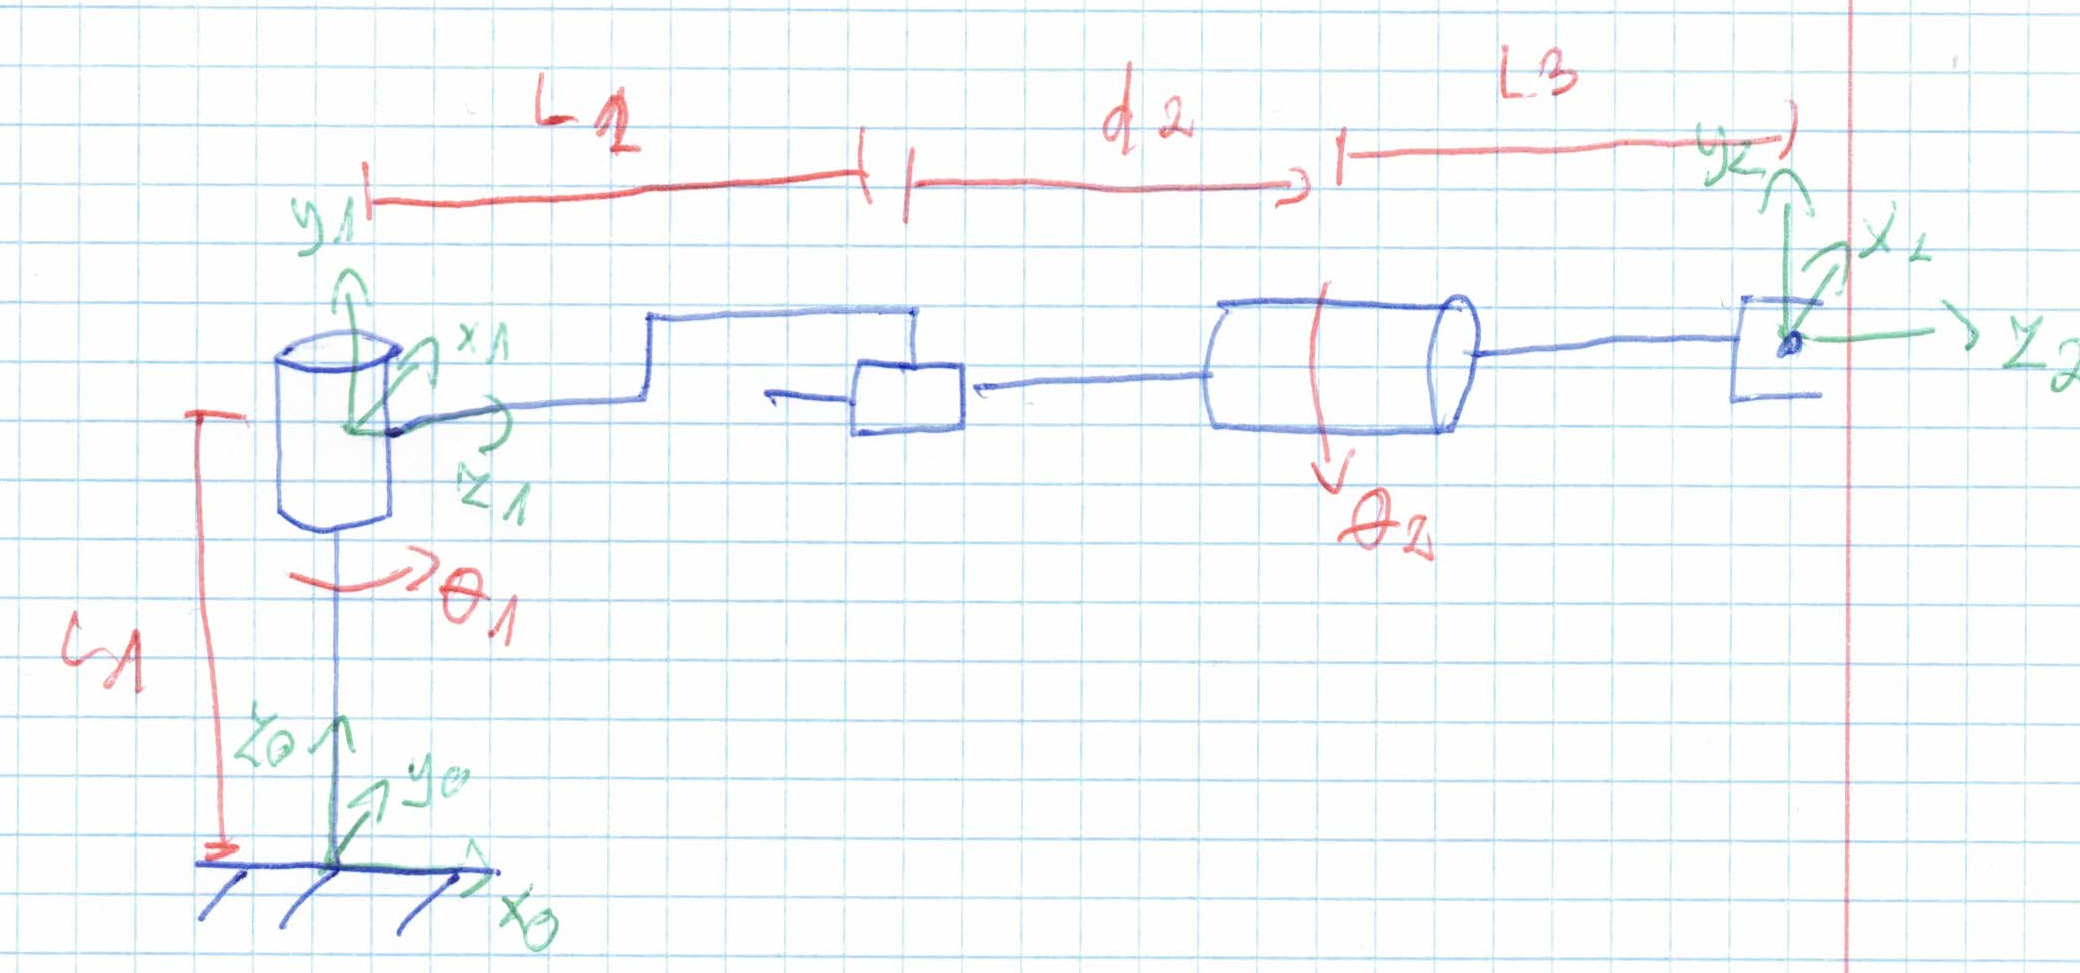
\includegraphics{src/rys_rob_DH.png}}
	\caption{Schemat robota} 
\end{figure}    
\begin{figure}[H]
	\centering
\begin{table}[H]
	\centering
\begin{tabular}{|l|l|l|l|l|}
\hline
i & \theta_{i} & d_{i} & a_{i} & \alpha_{i} \\ \hline
1 &  \theta_{1}+ 90   &l_1 & 0  &    90  \\ \hline
2 &   0& l_2+d_2   & 0  & 0     \\ \hline
3 &   \theta_{3} & l_3   & 0  & 0     \\ \hline
\end{tabular}
\end{table}
	\caption{Tabela DH} 
\end{figure} 

\begin{figure}[H]
\centering

$A^0_1=
\begin{bmatrix}
-s_1 & 0 & c_1 & 0 \\
c_1 & 0 & s_1 & 0 \\
0 & 1 & 0 & l_1 \\
0 & 0 & 0 & 1 
\end{bmatrix}  $
\end{figure} 

\begin{figure}[H]
\centering

$A^1_2=
\begin{bmatrix}
1 & 0 & 0 & 0 \\
0 & 1 & 0 & 0 \\
0 & 0 & 1 & l_2+d_2 \\
0 & 0 & 0 & 1 
\end{bmatrix}  $
\end{figure} 


\begin{figure}[H]
\centering

$A^2_3=
\begin{bmatrix}
c_3 & -s_3 & 0 & 0 \\
s_3 & c_3 & 0 & 0 \\
0 & 0 & 1 & l_3 \\
0 & 0 & 0 & 1 
\end{bmatrix}  $
\end{figure} 


\begin{figure}[H]
\centering

$A^0_3=
\begin{bmatrix}
-c_{3}s_{1}& s_{3}s_{1} & c_1 & c_{1}(l_2+d_2+l_3) \\
c_{1}c_{3} & -c_{3}c_{1} & s_1 & s_{1}(l2+d2+l_3) \\
s_3 & c_3 & 0 & l_1\\
0 & 0 & 0 & 1 
\end{bmatrix}  $
\caption{Macierz transformacji robota} 
\end{figure} 